% fig07_fodo_beta.tex — Twiss beta-functions beta_x, beta_y along one FODO
% cell (L_d=1 m drift, L_q=0.1 m quad, k1=0.25 m^-2). The Wiedemann/Lee
% thick-quad closed-form profile; Xsuite 0.51.1 tracks the same curve to
% rel err 2.7e-14 (beta_x_max), so the two are visually coincident -- the
% parity is reported numerically, not as a separable line. Compiled to PDF
% for Appendix D. Quad positions shaded.
%
% Data: thick-quad transfer-matrix propagation of the periodic Twiss
% solution. beta_x peaks at the focusing quad (s~1.05 m, ~83.63 m),
% beta_y at the defocusing quad -- the canonical FODO mirror pattern.
%
% Manual single-shot compile (debug):
%   xelatex -interaction=nonstopmode -halt-on-error fig07_fodo_beta.tex
\documentclass[border=4pt]{standalone}
\usepackage{tikz}
\usepackage{pgfplots}
\pgfplotsset{compat=1.18}
\begin{document}
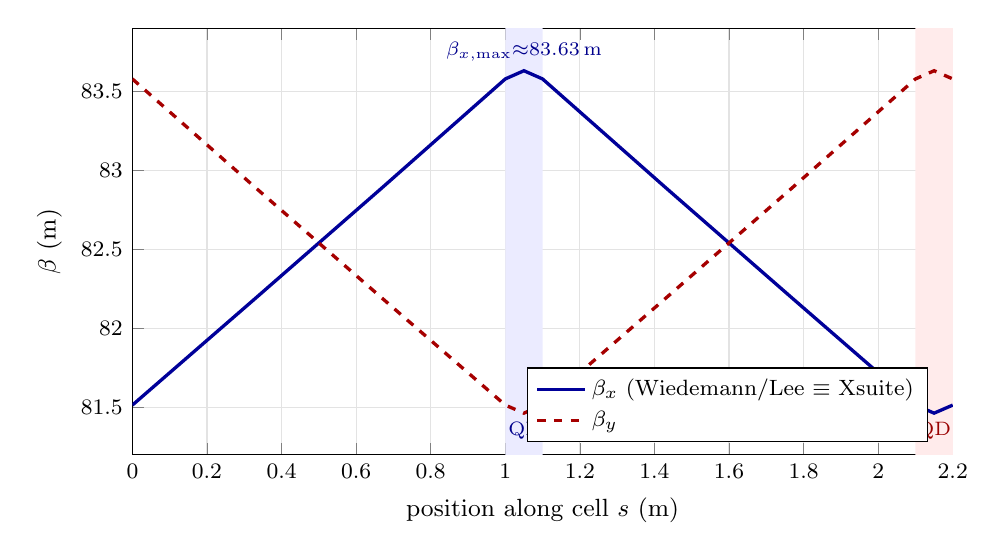
\begin{tikzpicture}
\begin{axis}[
  width=12cm, height=7cm,
  xlabel={position along cell $s$ (m)},
  ylabel={$\beta$ (m)},
  xmin=0, xmax=2.2,
  ymin=81.2, ymax=83.9,
  legend pos=south east,
  legend cell align=left,
  legend style={font=\footnotesize},
  tick label style={font=\footnotesize},
  label style={font=\small},
  ymajorgrids, xmajorgrids,
  grid style={gray!22},
]
% quad shading (QF at 1.0-1.1, QD at 2.1-2.2)
\addplot[draw=none,fill=blue!8,forget plot] coordinates {(1.0,81.2)(1.1,81.2)(1.1,83.9)(1.0,83.9)} \closedcycle;
\addplot[draw=none,fill=red!8,forget plot]  coordinates {(2.1,81.2)(2.2,81.2)(2.2,83.9)(2.1,83.9)} \closedcycle;
\node[font=\scriptsize,blue!55!black] at (axis cs:1.05,81.35) {QF};
\node[font=\scriptsize,red!60!black]  at (axis cs:2.15,81.35) {QD};
% beta_x
\addplot[blue!60!black, very thick] coordinates {
  (0.000,81.515) (0.333,82.197) (0.667,82.885) (1.000,83.579)
  (1.050,83.631) (1.100,83.579) (1.433,82.885) (1.767,82.197)
  (2.100,81.515) (2.150,81.464) (2.200,81.515)
};
\addlegendentry{$\beta_x$ (Wiedemann/Lee $\equiv$ Xsuite)}
% beta_y
\addplot[red!65!black, very thick, dashed] coordinates {
  (0.000,83.579) (0.333,82.885) (0.667,82.197) (1.000,81.515)
  (1.050,81.464) (1.100,81.515) (1.433,82.197) (1.767,82.885)
  (2.100,83.579) (2.150,83.631) (2.200,83.579)
};
\addlegendentry{$\beta_y$}
\node[font=\scriptsize,anchor=south,text=blue!55!black] at (axis cs:1.05,83.631)
  {$\beta_{x,\max}{\approx}83.63$\,m};
\end{axis}
\end{tikzpicture}
\end{document}
